\subsection{About MATLAB}
\begin{frame}{About MATLAB}
\begin{itemize}
\item Commercial and experience (Octave)
\item Not for general purpose (no one will write an operating system using MATLAB)
\item Excel at numerical calculations and plot
\item Many useful toolboxes (though we will not cover these in this course, you will use some of them in advanced courses)
\item Widely used in academia
\end{itemize}
\end{frame}

\subsection{Interface}
\begin{frame}{Interface}
\begin{figure}[htbp]
\centering
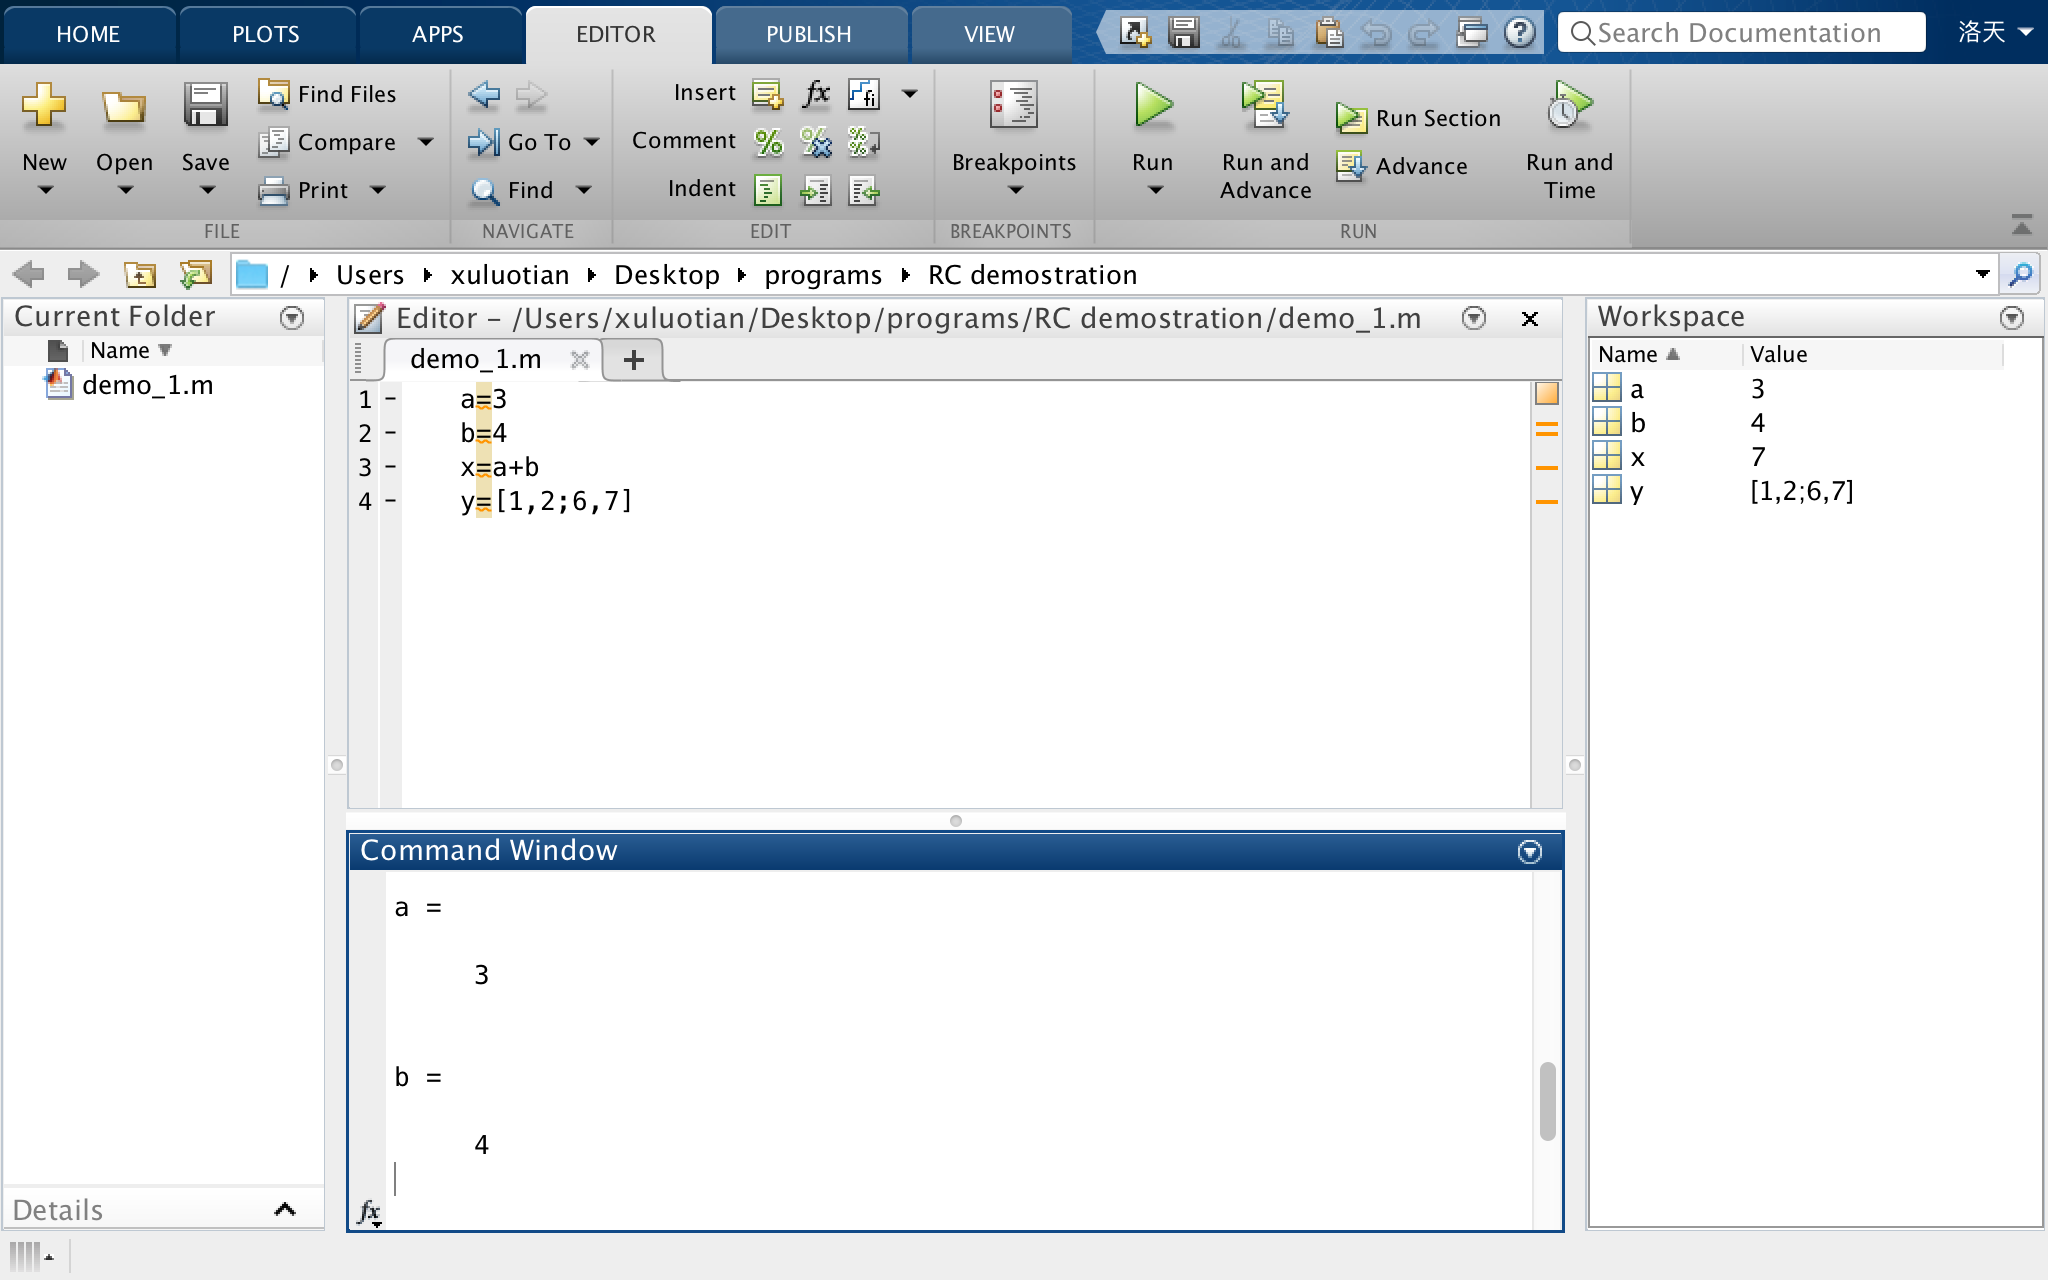
\includegraphics[width=0.95\textwidth]{pic/window.png}
\end{figure}
\end{frame}

\begin{frame}{Interface}
\begin{block}{Workspace}
Store and show what variables are available and their value. You can double-click a variable to see its details (useful for matrix). You can also save and load workspace.
\end{block}
\begin{block}{Command Window}
Input command direct into the command line. Variables can be seen in the workspace.
\end{block}
\begin{block}{Editor}
Editor is actually where you ``buffer'' your commands. \textbf{Run} the code in the editor is equivalent to type the command line by line into command window.
\end{block}
\end{frame}


\begin{frame}{Interface}
\begin{block}{Current Folder (\& Environment)}
It indicates which folder you are currently. When you operate on file (e.g. call a function from another file), MATLAB will search the file in current directory or search path. Personally, I suggest managing your file in the current directory, which will make your life easier.

For more details about search path, you can refer to \url{https://ww2.mathworks.cn/help/matlab/matlab_env/what-is-the-matlab-search-path.html?lang=en}.
\end{block}
\end{frame}

\begin{frame}{Interface}
Breakpoint: Useful tool for debugging.
\begin{figure}[htbp]
\centering
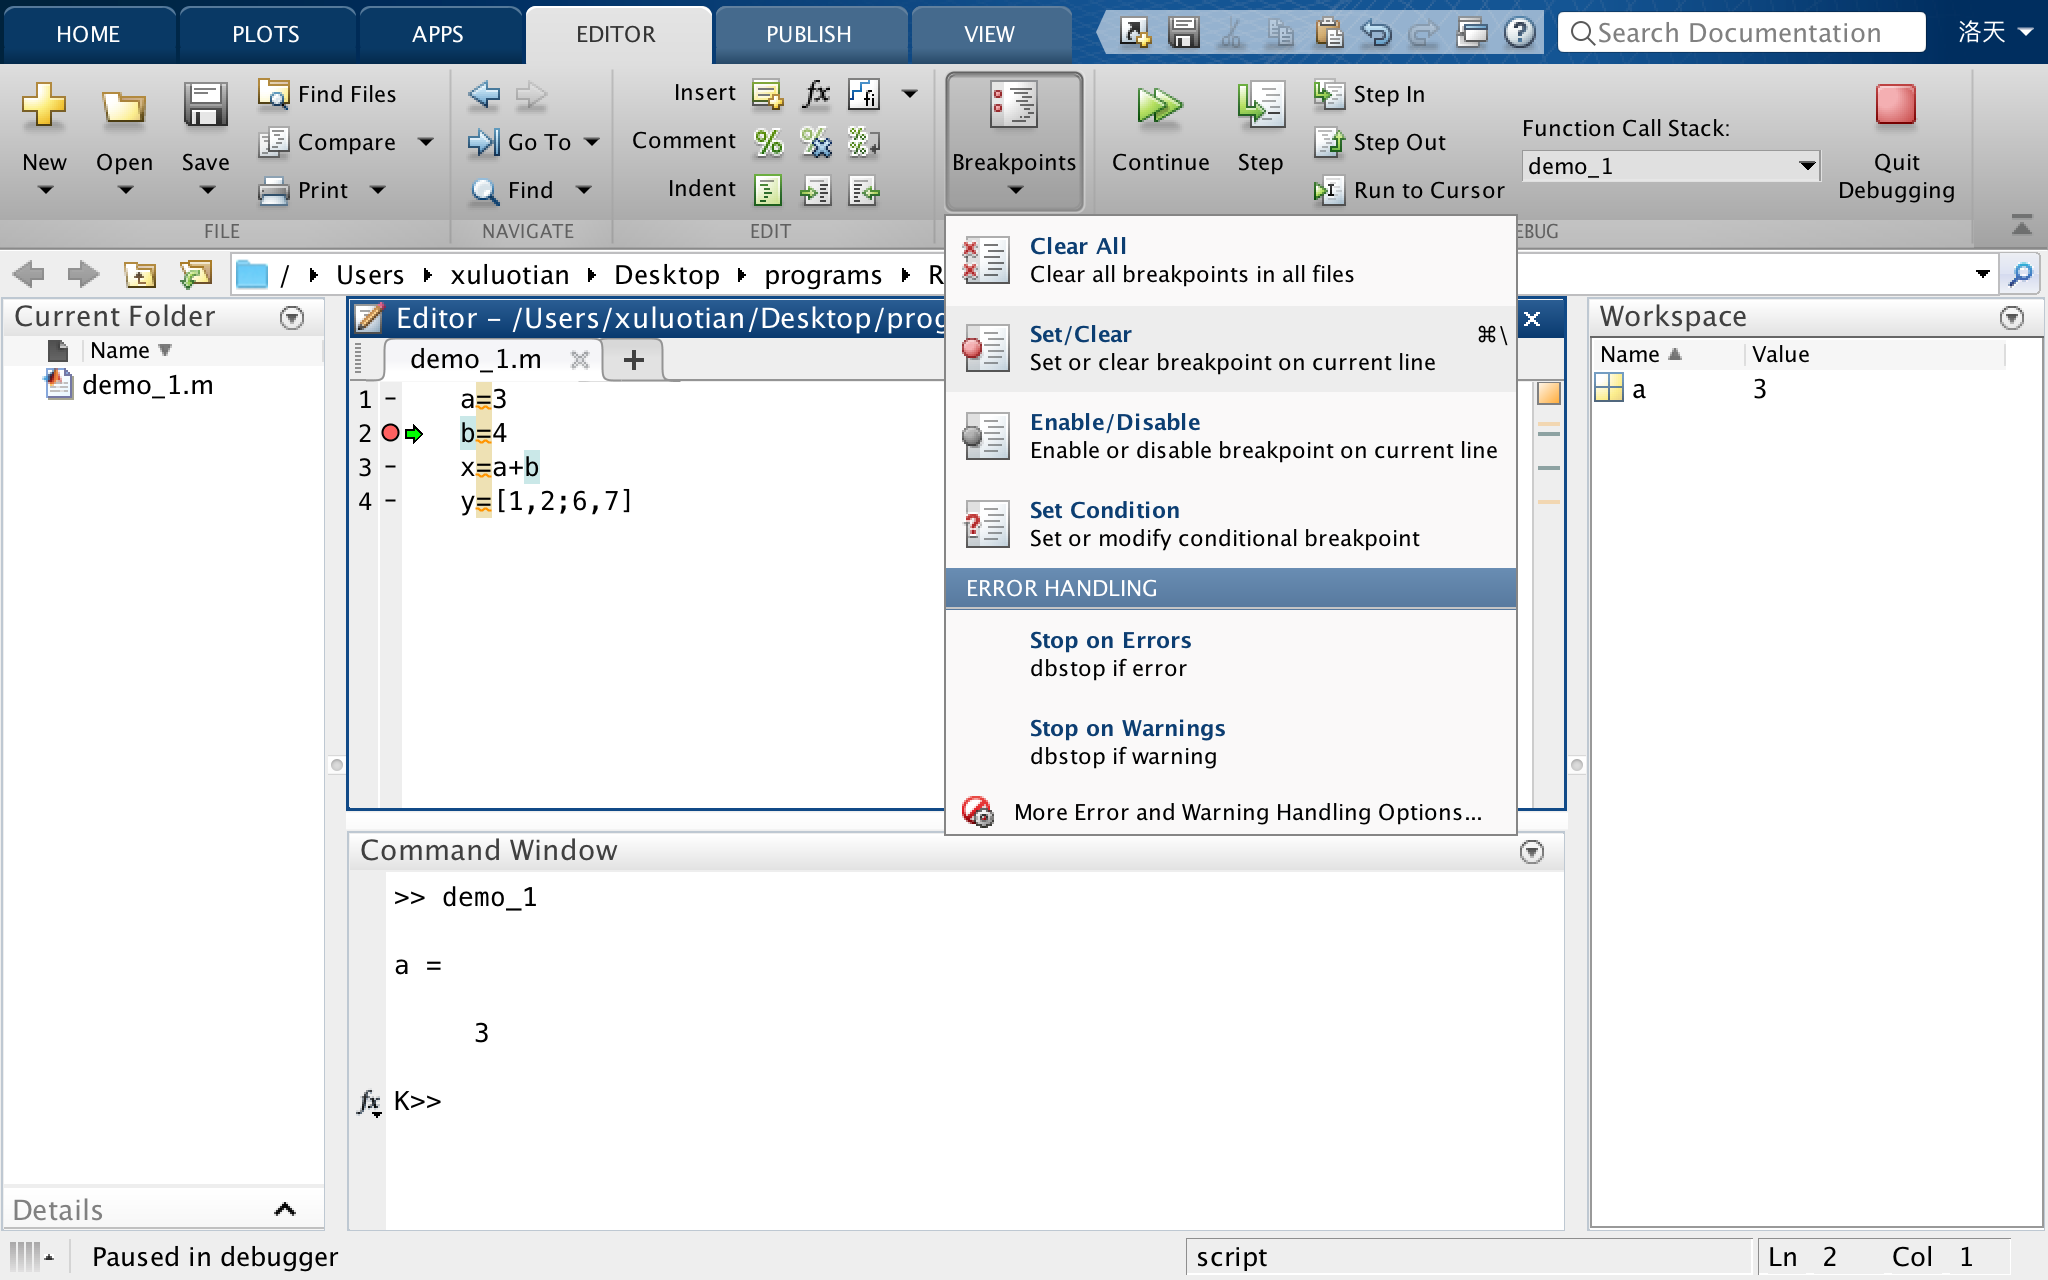
\includegraphics[width=0.9\textwidth]{pic/breakpoint.png}
\end{figure}
\end{frame}

\begin{frame}{Interface}
Documentation: Instructions for using MATLAB
\begin{itemize}
\item usage: doc / doc name (name = function you want to look up)
\end{itemize}
\begin{figure}[htbp]
\centering
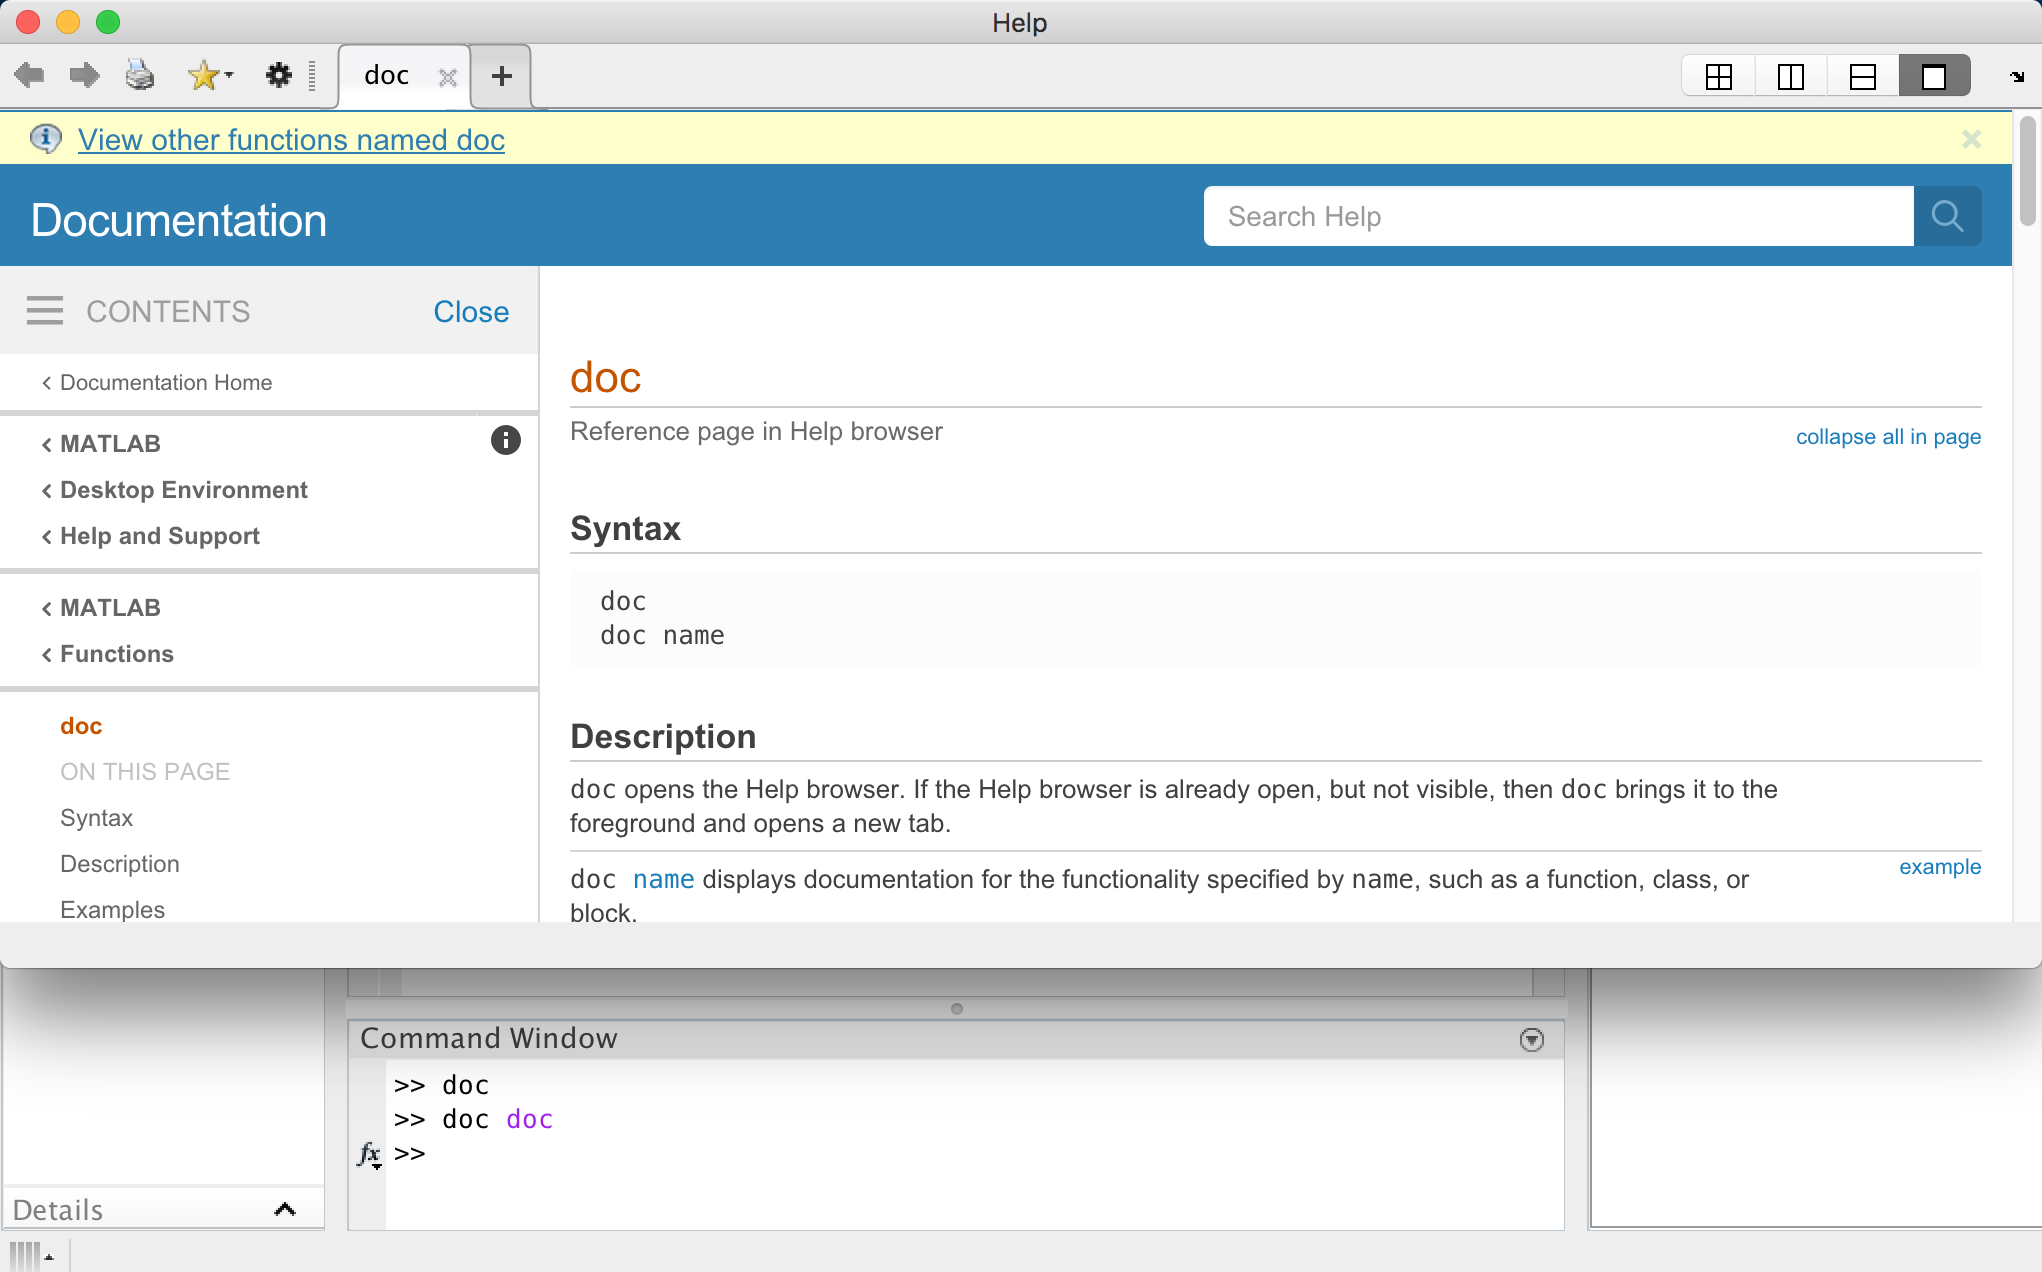
\includegraphics[width=0.8\textwidth]{pic/documentation.png}
\end{figure}
\end{frame}

\subsection{Syntax}
\begin{frame}{Operators \& Keys}
\begin{itemize}
\item ``+'', ``-'', ``*'', ``/'', ``.*'', ``./'', ``\ \^\ '', ``\ .\^\ '': matrix or element-wise arithmetic
\item ``='': assignment
\item ``=='': equal
\item ``\&\&'', ``$||$'': logical and / or
\item ``\%'': comment. Will be ignored by MATLAB. Make the code easier to understand
\item ``;'': suppress output. Please add it to every line that you do not expect output! Extra output may result in deduction
\item ``$\uparrow$, $\downarrow$'': view history
\item Tab: indent
\item ``clc'': clear command window
\item ``clear / clear all'': clear workspace
\end{itemize}
\end{frame}

\begin{frame}{Variables}
A valid variable name should
\begin{itemize}
\item Start with a letter (either upper or lower case)
\item Followed by letters/digits/underscores
\item Note that MATLAB is case sensitive
\end{itemize}
A good variable name should\footnotemark
\begin{itemize}
\item Have appropriate length (approximately 3 to 10 letters)
\item Self explain its function
\begin{itemize}
\item bad variable name:``a1'', ``a2, ``a3'', ``aa'', ``aaaa'', ``b'', ``c'', ``d''
\item good variable name: ``counter'', ``input'', ``flag''
\end{itemize}
\end{itemize}
Iteration variables ``i'', ``j'', ``k''
\begin{itemize}
\item Short, everyone use them
\end{itemize}
\footnotetext{Not required by VG101 but a really good habit.}
\end{frame}

\begin{frame}{Some Special Variables \& Constants}
\begin{block}{Tips}
\textbf{All variables in MATLAB are matrix.} Scalar is essential a $1\times1$ matrix, but it allows some operations that may be invalid for a $1\times1$ matrix.
\end{block}
\begin{itemize}
\item ``ans'': default output variable; do not use ``ans'' as your own variable name in your script
\item ``i'', ``j'': virtual number
\item ``Inf'': infinite
\item ``NaN'': not a number; mostly appear when the result exceed some limit or some errors occur
\item ``pi''
\end{itemize}

\begin{block}{Save \& Load}
\begin{itemize}
\item save xxx: save all current variables into .mat file
\item load xxx: load .mat file; will not clear variables already in workspace; will cover the variable in workspace if two variables share same name
\end{itemize}
\end{block}
\end{frame}

\begin{frame}{Command}
\begin{itemize}
\item ``exist'': test the existence of a varible or a file (exist xxx)
\item ``global'': declare global variable
\item ``help'', ``doc'': show document (help xxx; doc xxx)
\item ``clc'': clear command window
\item ``clear / clear all'': clear workspace
\end{itemize}
It's good habit to add ``clc'' and ``clear'' at the first of your program, \textbf{especially in your homework}.
\end{frame}

\begin{frame}{Data Types}
Variables has data types. Data type defines how your variable will store in computer. Basic data type you will use: 
\begin{itemize}
\item Integer (int8, int16, int32, int64)
\item Unsigned Integer (uint8, uint16, uint32, uint64)
\item Floating-point number (single, double)
\item Logical
\item Character
\end{itemize}
Default data type for any number variable is double.
\end{frame}

\begin{frame}{Data Types}
\begin{block}{Data type conversion:}
\begin{itemize}
\item new variable = data type (old variable)
\item for example: a = int8 (a)
\end{itemize}
Note: some information may be lost.
\end{block}
What will happen if we convert number to character?
\begin{itemize}
\item The ASCII code will be used!
\item The ASCII code build a bridge between character and integer.
\end{itemize}
\end{frame}

\begin{frame}{ASCII Code}
\begin{figure}[htbp]
\centering
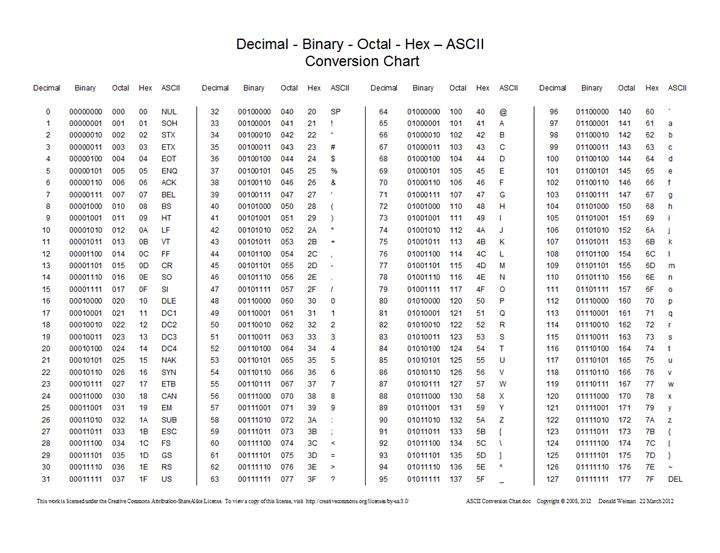
\includegraphics[width=0.9\textwidth]{pic/ascii.jpeg}
\end{figure}
\end{frame}

\begin{frame}{Matrix}
How to initialize array?
\begin{itemize}
\item A = [1, 2, 3; 4, 5, 6; 7, 8, 9]
\item A = zeros(3, 2) (row first, column next)
\end{itemize}
How to initialize matrix?
\begin{itemize}
\item A = [1:100] (step is 1 by default)
\item A = [0:0.01:1] (start, step, end)
\end{itemize}
MATLAB allows dynamic changes of array sizes. For example:
\begin{itemize}
\item A = [A; A]
\item A = [0, A] + [A, 0] (What can this do?)
\item A = [1: n];\\
	for i = 2 : n\\
	\ \ \ \ A = [A, [i: n, 1: i - 1]];\\
	end
\end{itemize}
\end{frame}

\begin{frame}{Matrix}
How to access an element of a matrix?
\begin{itemize}
\item A(2, 3) = The element at the second row and third column
\end{itemize}
How to access an element of a matrix?
\begin{itemize}
\item A(2) = The second element in A\\
\* If A is a 2-D matrix, it means the second element when arranging element of A by column
\end{itemize}
How to cut a sub matrix?
\begin{itemize}
\item Use ``:''  It is the most useful symbol in MTALAB.
\item A(: , 1) = the first column of A
\item A(1, : ) = the first row of A
\item A(1: 3, :) = the sub matrix consisting the first to third row of A
\item A(1: 3, 1: 3) = the upper-left corner 3 $\times$ 3 sub matrix of A
\item A(:, [i, j]) = A(:, [j, i])
\end{itemize}
\end{frame}

\begin{frame}{String}
\begin{block}{String}
When deal with words or sentences, MATLAB uses string. String is displayed in single quotation marks. String is not a new data type. It is a 1-D character matrix. Therefore, matrix operations all apply on strings.
\end{block}
Functions for string:
\begin{itemize}
\item strcmp, strrep, strfind
\item str2num, num2str, str2double
\end{itemize}
Check MATLAB document for usage of these functions.
\end{frame}

\begin{frame}
\begin{block}{Aside: Array \& Data Structure\footnotemark}
Array is the first and most basic data structure you will met. Data structure is a data organization, management and storage format that enables efficient access and modification.\footnotemark You can think of array as cabinet in our bathroom in D22/D21. Once you remember the number on the cabinet (for array, indices), you can quickly access the content in it. Array, regardless its dimension, is stored as a 1D sequence in memory. This enables convenient memory management and quick access. In latter courses, you will encounter more complicated data structures. 
\end{block}
\footnotetext{``Aside'' means the content below will be discussed in more advanced courses, but it can be quite helpful if you know it now.}
\footnotetext{Reference: \url{https://en.wikipedia.org/wiki/Data_structure}}
\end{frame}

\begin{frame}{M-file: Script \&Function}
Source code of MATLAB code is stored in .m files. It is essential text file, which means actually you can modify it as for .txt file. There are two kinds of .m file: script and function.
\begin{block}{script}
Scripts are essentially putting the code line by line to the command window. A script has no specific input and output. It operates on the value of workspace. Note that, if you do not clear the workspace before running a script, all variables in the workspace will be used by script, so of which are not intended, and may cause what you call ``XUANXUE'' (dark magic). \footnotemark
\end{block}
\begin{block}{function}
Functions take specific input and produce output. A function only working on its own varivables, which you can take it as a separate box. It promotes \textbf{code reuse} and \textbf{decoupling}.
\end{block}
\footnotetext{So you see why I mention adding ``clear'' in the front of your code is a good habit.}
\end{frame}

\begin{frame}{M-file: Script \&Function}
\begin{block}{Function syntax}
When defining:
\begin{itemize}
\item function [output1, output2 ...] = functionName (input1, input2 ...)
\end{itemize}
When calling (using):
\begin{itemize}
\item $[$output1, output2 ...$]$ = functionName (input1, input2 ...)
\end{itemize}
\end{block}
Note when using function:
\begin{itemize}
\item You should use same number of variables to accept the function output values, or the output with no variables to accept will be discarded.
\item If you don't specify the variable to accept the function output, MATLAB will create variable "ans" automatically, which is equivalient a single variable to accept function output.
\item Function name should be the same as the m file name. MATLAB will search file name to call the function.
\end{itemize}
\end{frame}

\begin{frame}{M-file: Script \&Function}
\begin{block}{Aside: Code Reuse \& Decoupling\footnotemark}
Code reuse not only means less code you need to produce; more importantly, it means less code you need to take care (debug, modify, or performance improvement). Decoupling means we would like the code be separated into modules, and limit the coupling only to the interfaces, i.e. where modules connect.
\end{block}
\begin{minipage}{0.48\textwidth}
	\structure{Low coupling:}
	\begin{figure}
		\centering
		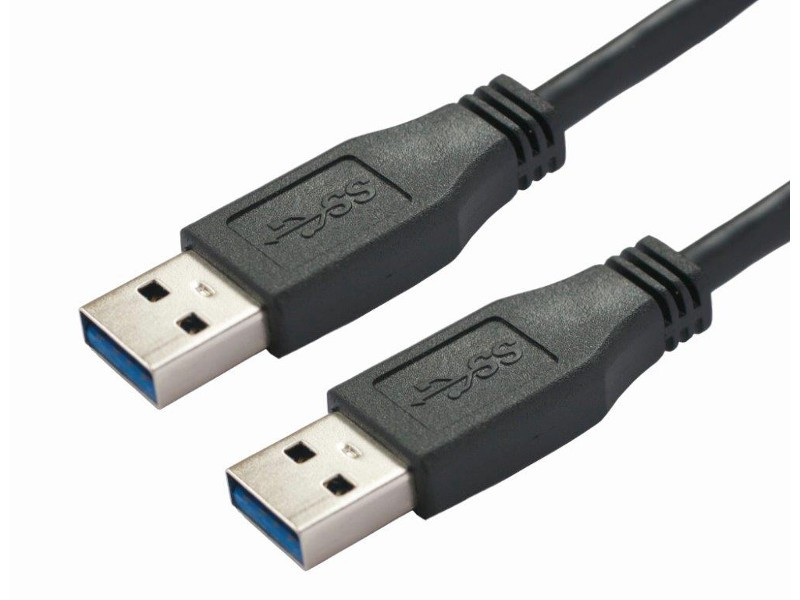
\includegraphics[width=0.4\textwidth]{pic/low-coupling.jpg}
	\end{figure}
\end{minipage}
\begin{minipage}{0.48\textwidth}
	\structure{High coupling:}
	\begin{figure}
		\centering
		
\includegraphics[width=0.4\textwidth]{pic/high-coupling.jpg}
	\end{figure}
\end{minipage}
\footnotetext{Reference and thanks: some of content is from \url{https://github.com/tripack45/VE280-Notes}.}
\end{frame}

\begin{frame}{Control Flow}
A computer program is like a factory that works on data. 
\begin{block}{Structured programming}
Three basic structures of computer programming
\begin{itemize}
\item sequencial structure
\item selective structure
\item cycle structure
\end{itemize}
Almost all tasks can be done using these three structures.
\end{block}
\begin{figure}
	\centering
	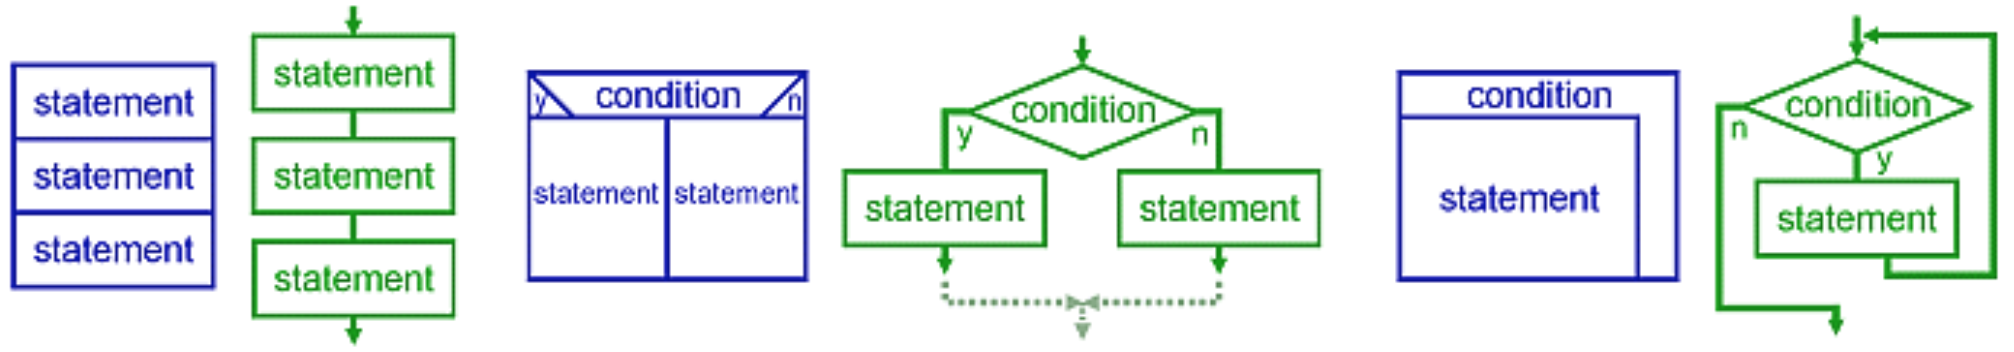
\includegraphics[width=0.9\textwidth]{pic/structure.png}
\end{figure}
\end{frame}

\begin{frame}{Control Flow}
\begin{itemize}
\item if, while, for
\item while 1
\end{itemize}
\begin{minipage}{0.05\textwidth}
~\\
\end{minipage}
\begin{minipage}{0.5\textwidth}
\lstinputlisting[language=Matlab]{code/control_flow_demo.m}
\end{minipage}
\begin{minipage}{0.05\textwidth}
~\\
\end{minipage}
\begin{minipage}{0.35\textwidth}
Outputs: \\
1 $\hookleftarrow$ \\
2 $\hookleftarrow$ \\
3 $\hookleftarrow$ \\
4 $\hookleftarrow$ \\
look, it is a four! $\hookleftarrow$ \\
5 $\hookleftarrow$ \\
100 $\hookleftarrow$ \\
99 $\hookleftarrow$ \\
98 $\hookleftarrow$ \\
97 $\hookleftarrow$ \\
96 $\hookleftarrow$ \\
\end{minipage}
\end{frame}

\begin{frame}{Control Flow}
\begin{itemize}
\item break: break the loop
\item continue: ignore the later code in this iteration; skip directly to the next iteration
\end{itemize}
\begin{minipage}{0.05\textwidth}
~\\
\end{minipage}
\begin{minipage}{0.5\textwidth}
\lstinputlisting[language=Matlab]{code/break_cont_demo.m}
\end{minipage}
\begin{minipage}{0.05\textwidth}
~\\
\end{minipage}
\begin{minipage}{0.35\textwidth}
Outputs: \\
9 $\hookleftarrow$ \\
6 $\hookleftarrow$ \\
5 $\hookleftarrow$ \\
4 $\hookleftarrow$ \\
3 $\hookleftarrow$ \\
\end{minipage}
\end{frame}

\begin{frame}{Input \& Output}
A = Input(``Please input: '');
\begin{itemize}
\item Most widely used for command window input.
\item Can be used to input anything you want, including matrix.
\end{itemize}
Other ways of Input: 
\begin{itemize}
\item fscanf: Used for file input, will be discussed later.
\item sscanf: Used for string input, not used currently.
\end{itemize}
For more information, you can refer to the help function.
\end{frame}

\begin{frame}{Input \& Output}
Not adding ``;'' outputs the value of an expression.
\begin{itemize}
\item Not recommended. You will receive deduction if you output redundant messages in homework by not adding ``;''.
\end{itemize}
disp(A);
\begin{itemize}
\item display the value of A with a new line
\item can display anything you want (number, string, matrix, etc.)
\end{itemize}
fprintf \& sprintf
\begin{itemize}
\item Both use format symbols
\item fprintf: print format message on command window/into file
\item sprintf: print format message into a string
\item fprintf = disp(sprintf)
\end{itemize}
\end{frame}